\section{Desenvolvimento}

\subsection{Estados de condução e formas de onda}

Adota-se $v_{dc}>0$, com as correntes $i_b$, $i_c$ e $i_{pv}$ orientadas dos armazenadores para os braços e a corrente $i_R$ orientada do barramento para a carga. Para cada braço $k\in\{b,c,pv\}$, define-se $s_k=1$ quando a chave inferior conduz ($Q_2$, $Q_6$ ou $Q_4$) e $s_k=0$ quando a chave superior conduz ($Q_1$, $Q_5$ ou $Q_3$). Como as chaves de um mesmo braço são complementares, $d_k=\overline{s_k}$ representa a razão cíclica da chave inferior, e $\alpha_k=1-s_k$ define a tensão do ponto médio, $v_{m,k}=\alpha_k v_{dc}$. Aplicando as leis de Kirchhoff, as tensões nos indutores resultam em
\begin{align}
v_{L_b}&=V_b-\alpha_b v_{dc},\nonumber\\
v_{L_c}&=v_c-\alpha_c v_{dc},\label{eq:vL}\\
v_{L_{pv}}&=V_{pv}-\alpha_{pv} v_{dc}.\nonumber
\end{align}
Dessa forma, com a chave inferior ligada o indutor é submetido a $V_k$ e, com a superior ligada, a $V_k-v_{dc}$. Dos $2^3=8$ estados possíveis, nenhum provoca curto-circuito, e todos estão listados na Tabela~\ref{tab:estados}.

\begin{table}[H]
\centering
\caption{Topologias de condução ($s_bs_cs_{pv}$)}
\label{tab:estados}
\footnotesize
\setlength{\tabcolsep}{3pt}
\begin{tabular}{llll}
\toprule
$s_bs_cs_{pv}$ & Chaves ON & Braços no barramento & $C_{dc}\dot v_{dc}$ \\
\midrule
000 & $Q_1,Q_5,Q_3$ & $b,c,pv$ & $i_b+i_c+i_{pv}-i_R$ \\
001 & $Q_1,Q_5,Q_4$ & $b,c$ & $i_b+i_c-i_R$ \\
010 & $Q_1,Q_6,Q_3$ & $b,pv$ & $i_b+i_{pv}-i_R$ \\
011 & $Q_1,Q_6,Q_4$ & $b$ & $i_b-i_R$ \\
100 & $Q_2,Q_5,Q_3$ & $c,pv$ & $i_c+i_{pv}-i_R$ \\
101 & $Q_2,Q_5,Q_4$ & $c$ & $i_c-i_R$ \\
110 & $Q_2,Q_6,Q_3$ & $pv$ & $i_{pv}-i_R$ \\
111 & $Q_2,Q_6,Q_4$ & nenhum & $-i_R$ \\
\bottomrule
\end{tabular}
\end{table}

Em cada intervalo, a derivada da corrente do indutor vale $V_k/L_k$ com a chave inferior ligada e $(V_k-V_{dc})/L_k$ com a superior ligada. Consequentemente, a tensão $v_{L_k}$ é uma onda retangular de dois níveis, a corrente $i_k$ é aproximadamente triangular, a corrente no capacitor do barramento é pulsada e a tensão $v_{dc}$, por ser sua integral, exibe ondulação em dente de serra por partes. A tensão do ultracapacitor, por sua vez, é a integral de $-i_c/C$, decrescendo na descarga e crescendo na recarga. Em regime periódico, impondo valor médio nulo para $v_{L_k}$, obtém-se
\begin{equation}
V_{dc}=\frac{V_b}{1-d_b}=\frac{V_{pv}}{1-d_{pv}}=\frac{V_c}{1-d_c},
\label{eq:ganho}
\end{equation}
sendo a última igualdade apenas quase-estacionária, pois $v_c$ varia ao longo da descarga. A ondulação pico a pico da corrente em cada ramo é dada por
\begin{equation}
\Delta i_{L_k}=\frac{V_k\,d_k}{L_k\,f_s}.
\label{eq:dI}
\end{equation}
A Figura~\ref{fig:ondas} apresenta, para três períodos PWM, os comandos das chaves inferiores, as correntes nos indutores e a tensão do barramento obtidos por simulação.

\begin{figure}[H]
\centering
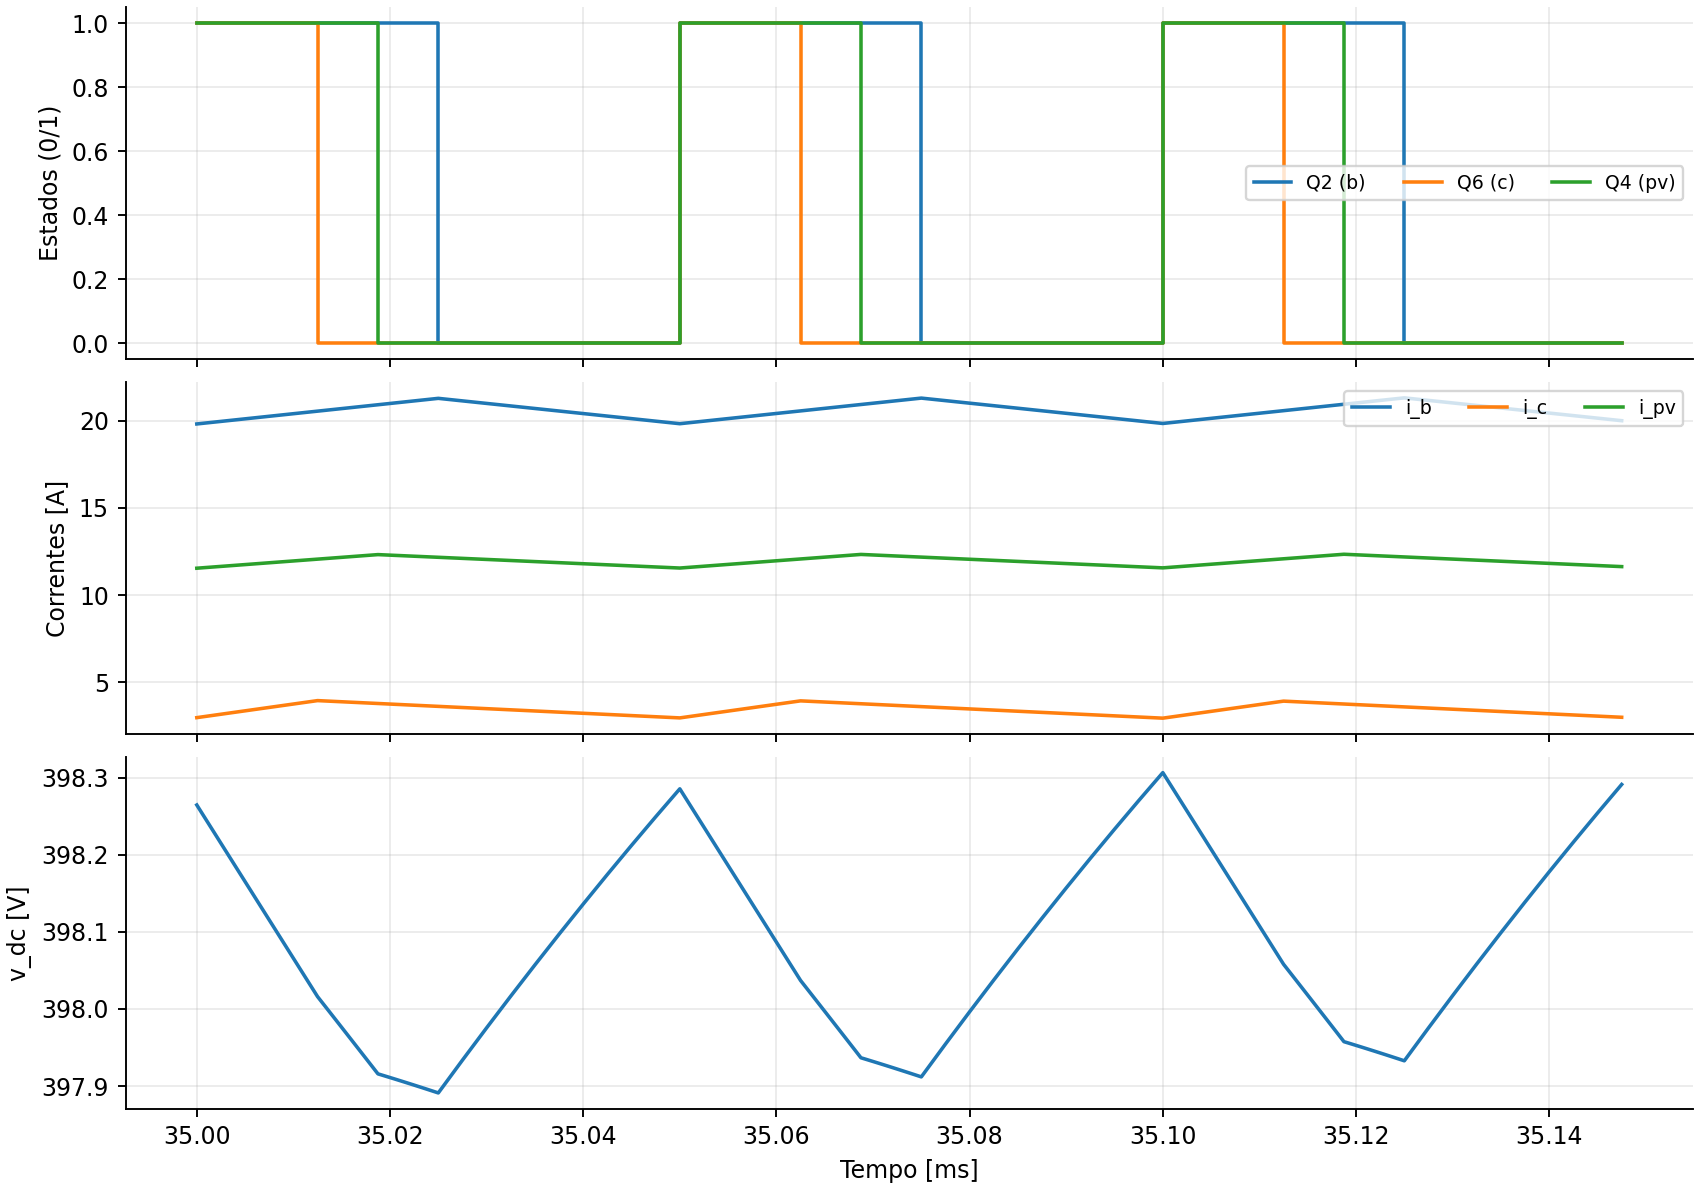
\includegraphics[width=\columnwidth]{images/fig_ondas.png}
\caption{Comandos das chaves inferiores, correntes nos indutores e tensão do barramento em três períodos PWM.}
\label{fig:ondas}
\end{figure}

\subsection{Dimensionamento dos componentes}

No equilíbrio permanente, $i_c=0$ e cada bateria entrega 4 kW, o que resulta em $I_b=20$ A e $I_{pv}=16$ A. Para que os três indutores sejam verificados simultaneamente, considera-se também um modo transitório no qual $P_b=3$ kW, $P_{pv}=2$ kW e $P_c=3$ kW, correspondente a $I_b=15$ A, $I_{pv}=8$ A e $I_c=10$ A. Como a ondulação relativa é maior quanto menor a corrente média, aplica-se \eqref{eq:dI} aos menores valores de corrente, exigindo ondulação de no máximo $10\%$:
\begin{align}
L_b&\ge\frac{200\cdot0{,}5}{0{,}1\cdot15\cdot20000}=3{,}333\ \text{mH},\\
L_{pv}&\ge\frac{250\cdot0{,}375}{0{,}1\cdot8\cdot20000}=5{,}859\ \text{mH},\\
L_c&\ge\frac{300\cdot0{,}25}{0{,}1\cdot10\cdot20000}=3{,}750\ \text{mH}.
\end{align}
Foram adotados valores comerciais ligeiramente superiores, resultando nas ondulações da Tabela~\ref{tab:dim}.

Para o capacitor do barramento, considera-se ondulação máxima de $20\%$, isto é, $\Delta V_{dc,max}=80$ V, e um limite conservador em que a carga descarrega o capacitor durante $d_{max}T_s=0{,}5\,T_s$:
\begin{equation}
C_{dc}\ge\frac{I_R\,d_{max}}{f_s\,\Delta V_{dc,max}}=\frac{20\cdot0{,}5}{20000\cdot80}=6{,}25\ \mu\text{F}.
\end{equation}
Esse limite refere-se apenas à ondulação em regime e não garante bom desempenho em transitórios de potência, razão pela qual se adotou $C_{dc}=1$ mF. Para o ultracapacitor, a capacitância é escolhida por energia e tempo de suporte, e não pela ondulação na frequência de chaveamento. Exigindo que $I_c=10$ A durante 0,5 s provoque $\Delta v_c\le0{,}2\cdot300=60$ V, obtém-se
\begin{equation}
C\ge\frac{I_c\,\Delta t}{\Delta v_c}=\frac{10\cdot0{,}5}{60}=83{,}3\ \text{mF},
\end{equation}
e adotou-se $C=0{,}1$ F, o que resulta em $\Delta v_c=50$ V e em energia liberada de 1375 J entre 300 V e 250 V. Ressalta-se que $d_c$ precisa ser ajustado continuamente à medida que $v_c$ muda, uma vez que a relação estática \eqref{eq:ganho} não pode ser mantida com $d_c$ fixo durante uma descarga prolongada.

\begin{table}[H]
\centering
\caption{Componentes adotados e ondulações obtidas}
\label{tab:dim}
\small
\begin{tabular}{lccc}
\toprule
Componente & Valor mínimo & Adotado & Ondulação \\
\midrule
$L_b$ & 3,333 mH & 3,4 mH & 9,80\% \\
$L_c$ & 3,750 mH & 3,8 mH & 9,87\% \\
$L_{pv}$ & 5,859 mH & 6,0 mH & 9,77\% \\
$C_{dc}$ & 6,25 $\mu$F & 1 mF & 0,08\% \\
$C$ & 83,3 mF & 0,1 F & 16,7\% \\
\bottomrule
\end{tabular}
\end{table}

\subsection{Modelo de espaço de estados}

Escolhendo o vetor de estados $\mathbf{x}=[i_b\ i_c\ i_{pv}\ v_{dc}\ v_c]^\top$, o modelo exato em cada intervalo de condução é
\begin{align}
L_b\dot i_b&=V_b-\alpha_b v_{dc},\nonumber\\
L_c\dot i_c&=v_c-\alpha_c v_{dc},\nonumber\\
L_{pv}\dot i_{pv}&=V_{pv}-\alpha_{pv} v_{dc},\label{eq:chav}\\
C_{dc}\dot v_{dc}&=\alpha_b i_b+\alpha_c i_c+\alpha_{pv} i_{pv}-\frac{v_{dc}}{R},\nonumber\\
C\dot v_c&=-i_c,\nonumber
\end{align}
que pode ser escrito como $\dot{\mathbf{x}}=\mathbf{A}(\alpha)\mathbf{x}+\mathbf{b}$, com as matrizes apresentadas em \eqref{eq:Amat}. Para cada uma das oito configurações da Tabela~\ref{tab:estados}, basta atribuir valores binários a $s_b$, $s_c$ e $s_{pv}$, enquanto o modelo médio em MCC corresponde à mesma expressão com $\alpha_k=1-d_k$.


\begingroup
\footnotesize
\setlength{\arraycolsep}{2.5pt}
\begin{equation}
\mathbf{A}=\begin{bmatrix}
0&0&0&-\dfrac{\alpha_b}{L_b}&0\\[7pt]
0&0&0&-\dfrac{\alpha_c}{L_c}&\dfrac1{L_c}\\[7pt]
0&0&0&-\dfrac{\alpha_{pv}}{L_{pv}}&0\\[7pt]
\dfrac{\alpha_b}{C_{dc}}&\dfrac{\alpha_c}{C_{dc}}&\dfrac{\alpha_{pv}}{C_{dc}}&-\dfrac1{RC_{dc}}&0\\[7pt]
0&-\dfrac1C&0&0&0
\end{bmatrix},\qquad
\mathbf{b}=\begin{bmatrix}\dfrac{V_b}{L_b}\\[7pt]0\\[7pt]\dfrac{V_{pv}}{L_{pv}}\\[7pt]0\\[7pt]0\end{bmatrix}
\label{eq:Amat}
\end{equation}
\begin{equation}
\mathbf{B}_d=\begin{bmatrix}
\dfrac{V_{dc}}{L_b}&0&0\\[7pt]
0&\dfrac{V_{dc}}{L_c}&0\\[7pt]
0&0&\dfrac{V_{dc}}{L_{pv}}\\[7pt]
-\dfrac{I_b}{C_{dc}}&-\dfrac{I_c}{C_{dc}}&-\dfrac{I_{pv}}{C_{dc}}\\[7pt]
0&0&0
\end{bmatrix},\qquad
\mathbf{B}_\ell=\begin{bmatrix}0\\0\\0\\-\dfrac1{C_{dc}}\\0\end{bmatrix}
\label{eq:Bmat}
\end{equation}
\endgroup

Como verificação de consistência, a energia armazenada, $E=\tfrac12\sum_kL_ki_k^2+\tfrac12C_{dc}v_{dc}^2+\tfrac12Cv_c^2$, deve satisfazer
\begin{equation}
\dot E=V_bi_b+V_{pv}i_{pv}-\frac{v_{dc}^2}{R},
\end{equation}
pois o termo $v_ci_c$ se cancela entre $L_c$ e $C$ por tratar-se de uma transferência interna, o que confirma os sinais adotados. Em seguida, linearizando em torno do ponto permanente $(I_b,I_c,I_{pv},V_{dc},V_c)=(20,0,16,400,300)$ com $(d_b,d_c,d_{pv})=(0{,}5,0{,}25,0{,}375)$, obtém-se
\begin{equation}
\dot{\hat{\mathbf{x}}}=\mathbf{A}(d_0)\hat{\mathbf{x}}+\mathbf{B}_d\hat{\mathbf{d}}+\mathbf{B}_\ell\hat i_\ell,
\label{eq:lin}
\end{equation}
com $\mathbf{B}_d$ e $\mathbf{B}_\ell$ dados em \eqref{eq:Bmat}, em que $\hat i_\ell$ é uma corrente incremental adicional extraída do barramento. Cabe destacar que, como $C\dot v_c=-i_c$, um equilíbrio estrito exige $i_c=0$, de modo que uma corrente não nula no ultracapacitor representa necessariamente um processo transitório de descarga ou recarga.

\subsection{Projeto do controlador \textit{droop}}

A estratégia de controle é composta por uma malha interna de corrente em cada indutor e por uma malha externa de tensão com característica de \textit{droop}, tendo sua implementação Figura \ref{fig:blocos}

\begin{figure}[H]
\centering
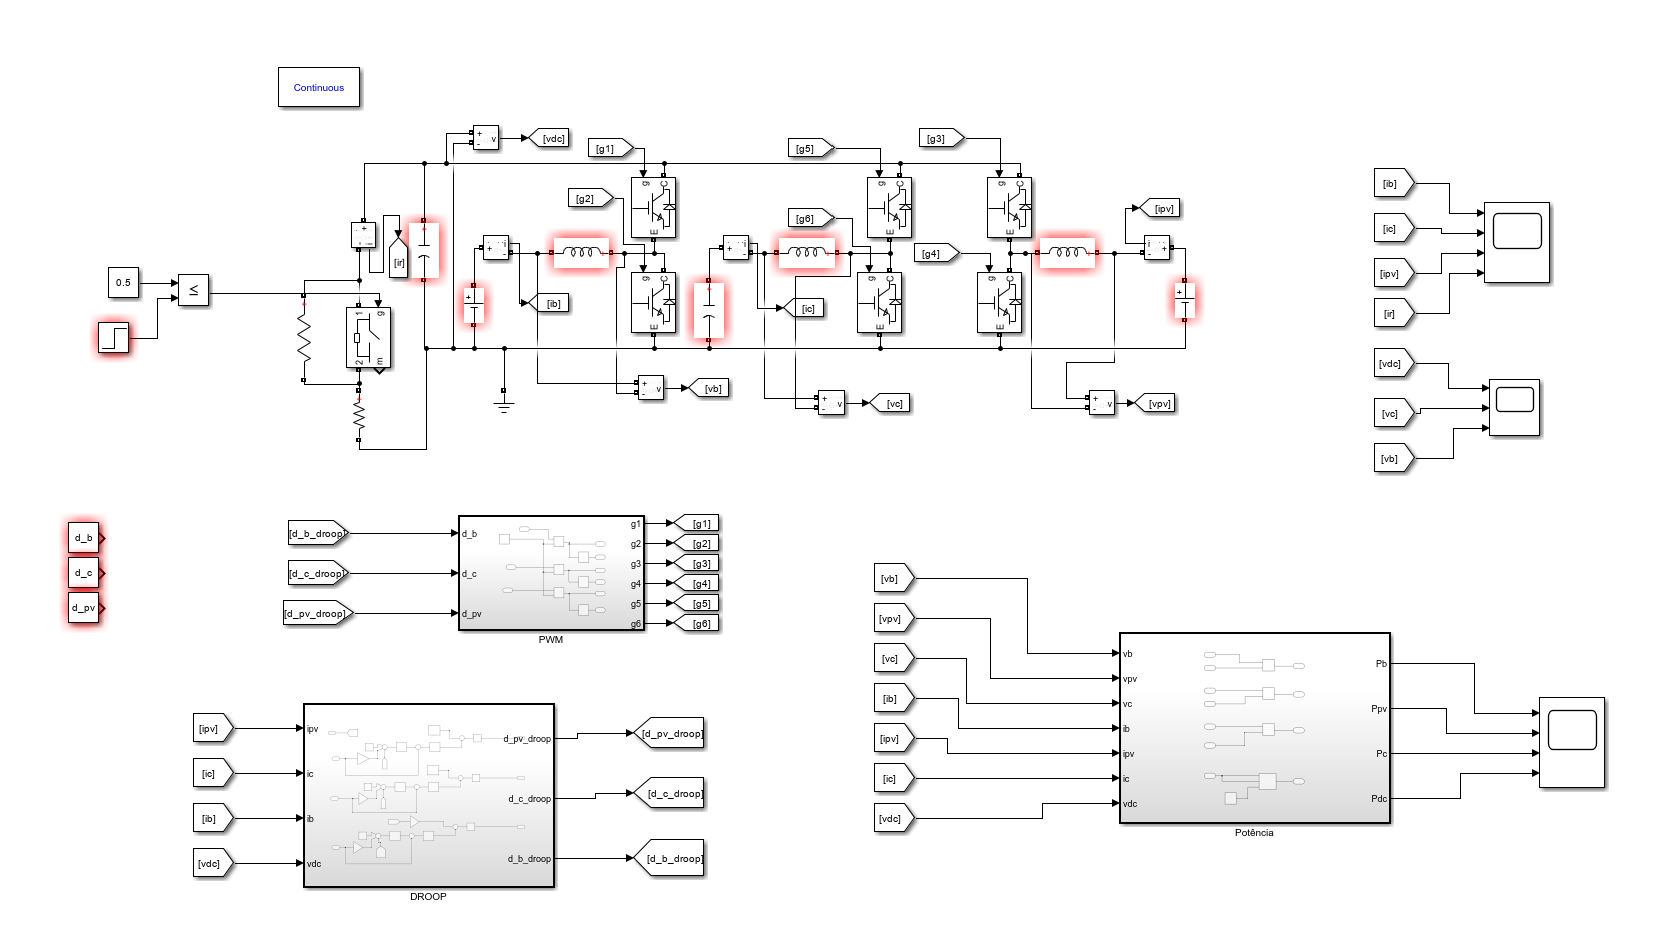
\includegraphics[width=0.9\columnwidth]{images/fig_diagrama_blocos.png}
\caption{Arquitetura do controle em dupla malha.}
\label{fig:blocos}
\end{figure}

Na malha interna, utiliza-se o \textit{feedforward} da tensão de entrada somado a um PI, com saturação das razões cíclicas em $[0{,}02;\,0{,}98]$ e anti-\textit{windup} condicional:
\begin{align}
d_k^{ff}&=1-\frac{V_k}{v_{dc}},\nonumber\\
d_k&=\mathrm{sat}\!\left[d_k^{ff}+K_{pi,k}\,e_k+K_{ii,k}\,\xi_k\right],\label{eq:pi}\\
e_k&=i_k^{\star}-i_k,\qquad\dot\xi_k=e_k.\nonumber
\end{align}
Com o \textit{feedforward} ideal, a planta vista pelo PI reduz-se a $\hat i_k/\hat d_k=V_{dc}/(L_ks)$, de modo que, escolhendo $\omega_{ni}=2\pi\cdot1000$ rad/s e $\zeta=0{,}707$, os ganhos são
\begin{equation}
K_{pi,k}=\frac{2\zeta\omega_{ni}L_k}{V_{dc}},\qquad
K_{ii,k}=\frac{\omega_{ni}^2L_k}{V_{dc}},
\end{equation}
cujos valores constam na Tabela~\ref{tab:ganhos}.

\begin{table}[H]
\centering
\caption{Ganhos da malha interna de corrente}
\label{tab:ganhos}
\small
\begin{tabular}{lcc}
\toprule
Ramo & $K_{pi}$ [A$^{-1}$] & $K_{ii}$ [(A$\cdot$s)$^{-1}$] \\
\midrule
Bateria 1 ($b$) & 0,07552 & 335,567 \\
Ultracapacitor ($c$) & 0,08440 & 375,045 \\
Bateria 2 ($pv$) & 0,13327 & 592,176 \\
\bottomrule
\end{tabular}
\end{table}

Na malha externa, a referência de tensão do barramento decresce com a corrente de carga, caracterizando o \textit{droop}:
\begin{equation}
v_{dc}^{\star}=400-r_d\,(i_R-20),\qquad r_d=1\ \Omega,\qquad i_R=\frac{v_{dc}}{R}.
\end{equation}
Definindo $e_v=v_{dc}^{\star}-v_{dc}$, a corrente total a ser entregue ao barramento é
\begin{equation}
J^{\star}=i_R+K_{pv}\,e_v+K_{iv}\,\xi_v,\qquad\dot\xi_v=e_v.
\end{equation}
Considerando a planta externa simplificada $1/(C_{dc}s+1/R)$, com $\omega_{nv}=2\pi\cdot40$ rad/s e $\zeta=0{,}707$, obtém-se
\begin{align}
K_{pv}&=2\zeta\omega_{nv}C_{dc}-\frac1R=0{,}3054\ \text{A/V},\\
K_{iv}&=\omega_{nv}^2C_{dc}=63{,}17\ \text{A/(V$\cdot$s)}.
\end{align}
Para que o ultracapacitor atenda preferencialmente aos transitórios e as baterias supram a potência média, a demanda é filtrada por $\tau_b\dot J_b^{slow}=J^{\star}-J_b^{slow}$, com $\tau_b=0{,}08$ s. Adotando partilha de $50\%$ entre as baterias, as referências de corrente dos indutores são
\begin{align}
i_b^{\star}&=\frac{0{,}5\,J_b^{slow}}{1-d_b^{ff}},\nonumber\\
i_{pv}^{\star}&=\frac{0{,}5\,J_b^{slow}}{1-d_{pv}^{ff}},\label{eq:refs}\\
i_c^{\star}&=\frac{J^{\star}-J_b^{slow}}{1-d_c^{ff}},\nonumber
\end{align}
em que o fator $1-d_k^{ff}=V_k/v_{dc}$ converte a corrente média desejada no barramento em corrente de indutor. Trata-se de uma escolha de gerenciamento de energia, não da única possível, uma vez que, na prática, exigem-se também limites de temperatura, estado de carga, corrente e potência dos bancos.